\documentclass[10pt,draftclsnofoot,onecolumn]{IEEEtran}
\usepackage[letterpaper, portrait, margin=0.75in]{geometry}
%\usepackage[myheadings]{fullpage}
\usepackage{fancyhdr}
\usepackage{lastpage}
\usepackage{graphicx, wrapfig, subcaption, setspace, booktabs}
\usepackage[T1]{fontenc}
\usepackage[font=small, labelfont=bf]{caption}
%\usepackage{fourier}
\usepackage[protrusion=true, expansion=true]{microtype}
\usepackage[english]{babel}
%\usepackage{sectsty}
\usepackage{url, lipsum}
\usepackage{tikz}
\usepackage{listings}
\usepackage{placeins}

\newcommand{\namesigdatehrule}[1]{\par\tikz \draw [blue, densely dotted, ultra thick] (0,0) -- (#1,0);\par}
\newcommand{\namesigdate}[2][5cm]{%
\begin{minipage}{#1}%
    #2 \vspace{0.8cm}\namesigdatehrule{#1}\smallskip
    \small \noindent\textit{Signature}
    \vspace{0.8cm}\namesigdatehrule{#1}\smallskip
    \small \textit{Date}
\end{minipage}
}


\newcommand{\HRule}[1]{\rule{\linewidth}{#1}}
\newcommand*\tick{\textsc{\char13}}
\singlespacing
\setcounter{tocdepth}{5}
\setcounter{secnumdepth}{5}


\begin{document}
%\title{HyRo}
%\author{Jason Klindtworth  |  Josh Asher  |   Layne Nolli}
%\date{}
%\maketitle
\begin{titlepage}
	\centering
	{\scshape\LARGE HyRo \par}
	\vspace{1cm}
	{\scshape\Large Jason Klindtworth  |  Josh Asher  |   Layne Nolli\par}
	\vspace{1.5cm}
	{\huge\bfseries CS463\par}
	\vspace{2cm}
	{\huge\bfseries Team 28\par}
	\vspace{2cm}
	{\Large\itshape Spring 2017\par}
	\vspace{4cm}
	{\Large\itshape Spring Midterm Progress Report\par}
	\vspace{4cm}
	{\large Abstract\par}
	\vspace{1cm}
	Half way through our last term in capstone we have accomplished a lot and are proud of what we have done. This has been a very busy term and we have
	needed to finalize our project, finalize our poster, and prepare for our expo presentations. Everything has been completed on time and testing with the ECE team has occurred. We present to you a report on the current status of our project and what small things we have left to do. As well as a look back on problems we encountered and how we managed to solve them.\par

	\vfill

% Bottom of the page
	{\large \today\par}
\end{titlepage}


\section{Overview of Purpose and Goals}
OSU has for the past 2 years had seniors from MIME and ECE develop a hybrid rocket for their capstone projects. The first years didn't even get off the ground, but through their efforts lasts years team was able to build a hybrid that went 5000 feet. They were able to build a system to collect a large amount of data from on-board sensors, but had no way to easily visualize it. That's why we were asked to join the project this year. This is the first year a CS team has worked on the hybrid rocket team. Our goals are to provide visualization to their data along with providing remote controls (like filling the oxidizer tank) to allow the team to operate the rocket entirely from a safe distance. Through the course of this project we have had to work closely with the ECE team that is also part of this project. We were giving fairly free operating parameters and had to make many decisions on our own. Whatever the ECE team has been able to provide us we have been able to visualize. \par

In the last two terms we did a lot of prototyping and requirement changes. Originally we were supposed to control more aspects of the rocket operation remotely. Over the course of the last term we were informed by the ECE team that many of the operations we had planned (like arming, launching) were not going to be available through their avionics bay. So we had to downsize that portion of our project. That is ok and we hope by the time we launch we get a little of this functionality back, but for now our main goal as far as remote controls go is operating the remote filling. Our goals last term were to get a working beta out and we succeeded in that, but hadn't got as far as integration testing, including testing the software with real data. This term has been a little different. \par

Goals for this term include(d) finalizing all paper work, finalizing the code, integration testing, removing any major bugs, making a poster, preparing for expo, and then participating in expo. Further than that we look forward to our rocket launch. This has been a major issue because our rocket isn't even assembled yet, let alone the motor being tested. As this has come along further we have been requested to perform a couple stretch goals. One being the ability to inform the user that the parachute has been deployed and another to provided a GPS vector to where the rocket lands. We are almost done with both of these stretch goals, but they will not be part of our expo presentation. Another goal is to provided something entertaining at expo. At the moment we are going to record a video with some data from the ECE team, but hopefully we can demonstrate the software live in some way at expo in coordination with the ECE team. \par

We have done very well over the course of these last few terms. We have reached all the requirements laid out for us, even though some were taken away. The biggest question we have is will it actually work at launch. We wont be able to find out till it happens, but obviously this is our biggest goal looking forward. We have confidence that the equipment will work, but its a little nerve racking when you have a rocket that will go Mach 1.7 and your crossing your fingers the radio communication will hold. Wish us luck! \par

\section{Where We Are Currently and Where we Need to Head}
At this point in the project we are technically finished with the software. There is however some stretch goals that have been requested that we can complete after expo before the launch. First lets recap paper work and expo stuff. We had to do some final revisions to our requirements and design document. First of the requirements document had some lingering things we were not responsible for any more. The ECE team actually accomplished all of the on board rocket software so we did not have to write any of that. We coordinated as far as making sure our software would work with theirs but they built that part of the system. We have our own beagle bone and XBees to work with so we did write some test code for checking that our program worked. But that was out the requirements spec. We also had to delete some of our buttons we originally had in the requirements spec. This happened because last years team members tried to give us what they thought the requirements where going to be, but were not part of this years team. So when the rocket was getting designed they neglected to have our ECE team or us put some of the remote control abilities last years guys wanted. They did not need us to do those. It was a big miscommunication, the project was almost entirely student driven and we did not get good information for a while. This did not effect the fill control, visualization, replaying, or logging of the data. \par

We had to change our design document because of the requirement changes. That included commenting out those buttons we no longer needed. During development we also needed to change the flow of data so that was updated in the design document. Our original idea was not efficient and we discovered python queues which worked perfectly for our situation. This was updated in that document as well.\par

One of the biggest things this term is the infamous expo. We have completed our poster and have had it approved as well as practiced our expo speeches. To prepare for expo we have gathered some sample data we will record in a video that will be on repeat on a laptop during the expo. We hope to be able to hook up the avionics bay live at expo, to have a little fun in showing our stuff off. We are limited to battery life on the bay so this might not be possible. All in all we are pretty much ready for expo besides a nice shirt and hair cut. \par

As far as our software is concerned we are finished with it for expo. There will be a little more added for the team before the launch. We took the first couple weeks of this term to get our code finalized, commented, and a read me made. At the begging of the term we had a working interface, but there were a few missing things and some major tweaks to do. First of all we re-worked the graphics of the interface, buttons, and gauges. It looks awesome now, kinda silly in tone, but it fits the hybrid team well. We added tick numbers to the tick marks on the gauges so you know what the value is. This was missing and very essential. We realized over the course of last term we needed the ability to start and stop communications as well as log these sessions. We got this implemented and working very well. Now every time you click on start it will initiate the XBee and begin receiving data. This data is then logged in a folder under the data directory marked with a time stamp. This provided us an easy way in to complete our goal of replaying data. We added the load button where you can select a time stamped directory in the data directory that will repopulate the graphs with data from that run. Very awesome! \par

We had to adjust our sending routing to match the API the ECE team was using, but that proved to be fairly easy. One major bug we had we just fixed the other day was a memory leak. This thing was bad and we didn't notice until we ran the program through a loop for a long time. It was taking all the memory on the system! This was due to the fact we were not clearing our graphs correctly. We figured this out after a couple hours of banging our heads and the memory leak is gone. \par

From here on out there are a few things to accomplish. We need ot experience expo, do our final paper work and reports, add a few things to the software that were stretch goals, and launch this darn rocket! We are going to do another round of integration testing with the ECE team next Monday in the library, to make sure there are no bugs to work out between us. This will probably happen a few times before launch also. We want things to go really smooth with the rocket launch. We also are going to integrate the parachute deployment notification since the ECE team now can send us that information. GPS is going to be provided now apparently and we are developing a separate scheme to track the rocket. This is going to be simple unless we have time to do something more complex. We just plan on taking GPS coordinates at our station and comparing them to the coordinates coming in from the rocket. The ME teams might add a couple more controls to the rocket and if the ECE team also adds to their avionics bay we will provided any necessary functionality in our software for the team. \par

\section{Major Problems And Solutions}
We are nearing the end of this 3 term long project and there is a lot of anxiety about finishing everything and having a good working piece of software. Everyone is extremely busy an mostly on there last term of school so classes are rather intense. This lack of time issue has haunted us the entire senior design course. As always we find ways to make time for the project and get things done. This is usually done in spurts, but this term we have a major hold on how to get what we need done. Nancy again is hard to get a hold of. She is a very nice lady, but a very busy one. Having about 5 rocket teams to be in charge of is quite daunting and its hard to find here to get approval on things. We almost had a major poster disaster and she informed us the day after the submission deadline that we needed a certain logo on the poster. Luckily this was remedy by a little quick thinking and we will be placing a placard in front of our poster with AIAA logo on it. For some reason this information did not trickle down to the team even though we have been attending all meetings. \par

Our project was not finished when the term started. We had some important things to implement still. We got around this by working our butts off at the begging of the term. It really wasn't that bad and the final pieces came together quickly. In fact our solution to logging data made replaying data super easy. We didn't even think of doing it that way, but it kinda fell in our laps. We did not like the state of our graphics, but also conquered that in the major round of coding we did. Like I mentioned above the biggest problem with our software was the memory leak. We found this one day when we were testing for a long period of time. Our program would just eat up the RAM on the system. This took us a while, but to find out where the memory was leaking we employed the classic comment out move. We would block off section of the code to see where the memory leak was coming from. First we tried the XBee and that wasn't it. Then we tried the gauges, that wasn't it. Finally we commented out the graph redrawing and memory leak went away. We narrowed the redraw down to one graph and then tinkered with it until we realized we were not deleting old objects. Since the program redraws a lot these object were piling up in memory. We fixed this by properly destroying these objects.\par

Another major issue was that the ECE team was nearly impossible to get a meeting with. They have lab during the rocket meeting times and we didn't get to do much integration testing. This has changed recently and have tested our system with them. More tests are to be done next Monday and we have been insisting on more times to test. This persistence has payed off and we have a few meetings planned to test the system as a whole. We want a very smooth launch day when it comes up. \par

One of our major software related problems is and will be the lack of data. We have some data from last year, but it is hard to fake launching a rocket. Measuring data from a avionics bay that is stationary will not give us an accurate representation of what it is going to look like live. The ECE team luckily tested the bay in a barometric chamber and recorded all the data. We have been using this data to test our software and it is working great! \par

\pagebreak
\section{Interesting Piece of Code}
Last time we showed our Xbee radio transceiver class. This time we wanted to show you our function that converts the acceleration data into velocity data. Its not super complicated, but we were impressed at how easy it was to find a python library that did numerical integration. This function reads the acceleration data from a file, puts it into an array, and then passes it to Scipy's numerical integration function. Then the results are placed into the velocity data log with a time stamp. This is later used by the velocity redraw function to graph velocity. We thought this part of the project would be much more complex, but turned out to be rather efficient and not hard to code. \par

\begin{lstlisting}
#This function will convert the acceleration data into velocity data using scipy's numerical integration.
def convVel(value, directory):
#open acceration data file and read in contents
j = []
k = []
readFile = open(directory+'ASample.txt', 'r')
sepFile = readFile.read().split('\n')
readFile.close()

#need enough points to integrate
if(len(sepFile) < 3):
pass

else:
# add values to array to integrate
for plotPair in sepFile:
if(plotPair == ""):
continue
aAndB = plotPair.split(',')
j.append(float(aAndB[0]))
k.append(float(aAndB[1]))
#Uses simpsion functino to numerically integrate the acceration data
data = integrate.simps(k, x=j)

t = round(time.clock()) #get clock time for value
#open and write velocity data to VSample.txt for use by the velocity redrawing function
file = open(directory+"VSample.txt", "a")
file.write("\n")
file.write(str(t)+","+str(data)); 
file.close()
#print("Velocity: " + str(data))

\end{lstlisting}
\pagebreak

\section{Current Screen Shot}
This is our final GUI we will show at expo. Minor changes might take place before the rocket launch. \par

\begin{figure}[!ht]
  \caption{Screen shot of the graphical user interface.}
  \centering
	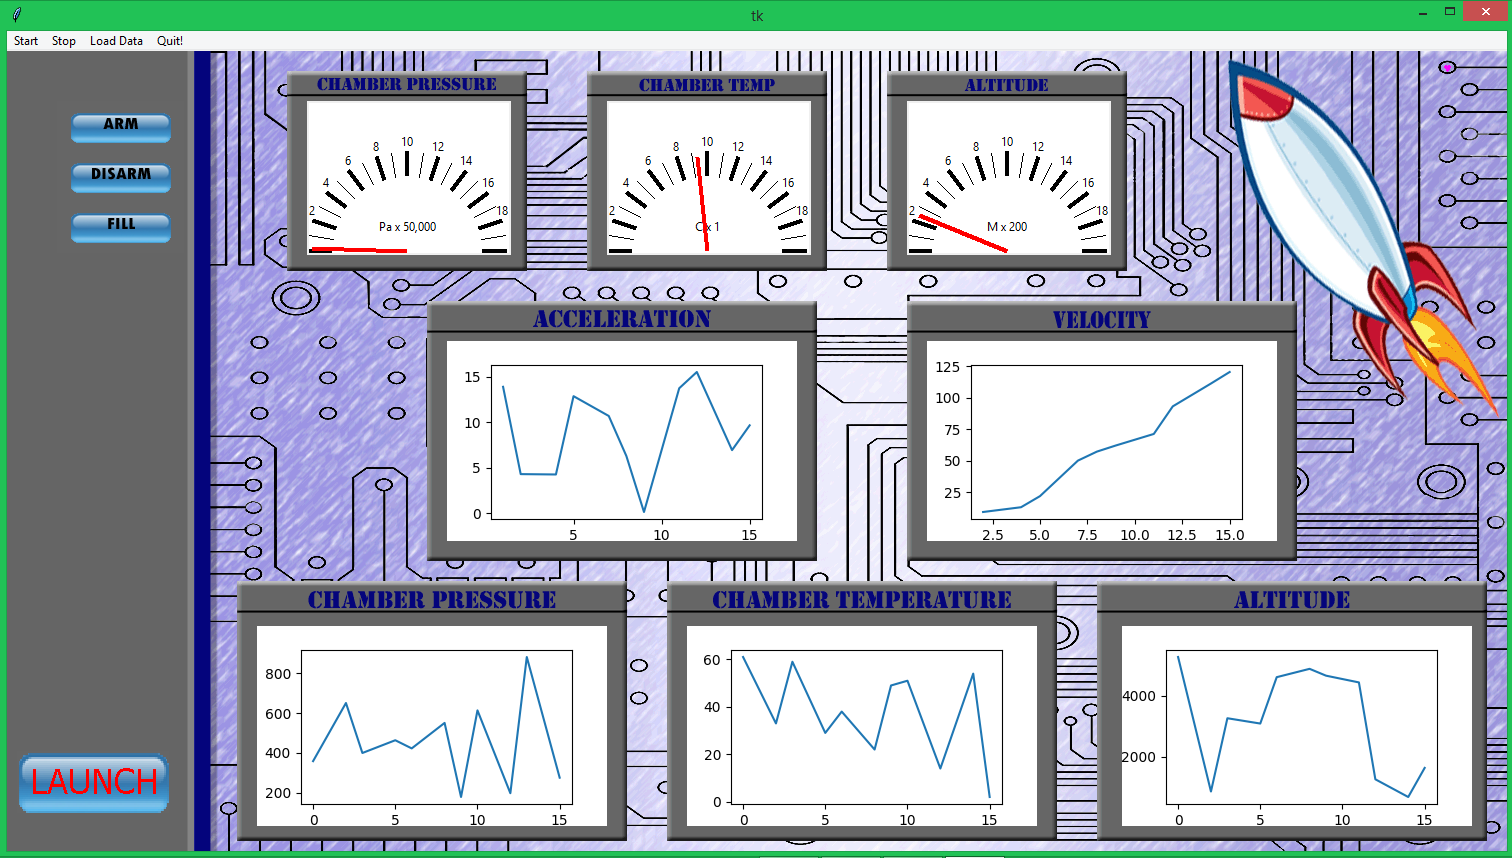
\includegraphics[scale=.40]{HyroGui}
\end{figure}
\FloatBarrier

\section{User Studies}
We have a very narrow group of users that will be using our project. Of course we hope that next year they can take our code our ideas and build off that. For now our users will be the Hybrid Rocket team. There is about 15 of us and we have been showing the GUI at the rocket meetings on Wednesday. Its reception has gone well and everyone says its easy to under stand and use. They did request a couple more data items to show up on the screen, but we are working on these are stretch goals. They said the graph data was easy to read and the gauges added a nice flair. They were impressed that we could load old data and found it very easy to use. All in all we got good rating from the team and we are still working with them to see if they want any more changes.\par

\section{Week by Week Recap}
The following is a week by week recap from each team member up to week 6 of spring term.  \par

\subsection{Week 1}
\subsubsection{Josh Asher}
 We have not made any progress on the project since last term. We have wrote a list of things we need to get done which is not to numerous. We need to tweak some graphics and tweak the logging mainly. Our beta is still running great though. Plans - Our biggest plans are to meet with the electrical engineers and run some real tests. We will be meeting the entire group next Wednesday and arranging for this to happen. We most likely will need to meet a couple times to get everything hammered out. We also are going to email Nancy to make sure we can use the Hybrid logo on our poster. We also will be doing updates on our poster this week and next week to get ready to present it to Nancy. We need to prepare for expo and are hashing out plans for that. Problems - We haven't come up with a lot of new problems. Mainly just finishing what we need for expo and the project. Our rocket is not built yet if you want to consider that a problem and we haven't fully tested real data. We plan on hashing this out next week and the week after. \par

\subsubsection{Jason Klindtworth} 
We did not get any work done over spring break, but we all agree that we are ahead of the game in the overall project so we were not really worried about it. We should be on track to make some good progress in the first part of this term. Josh broke his computer over the break so he is working on getting the development environment back up and running on his system. I am working on polishing the new graphics that we are going to be using for the final version of the software. We need to collaborate with the ECE team in order to get some real data that we can use for testing, but that will happen hopefully later this week or next week.\par

\subsubsection{Layne Nolli}
Project is still in an "almost complete" state from last term. We didn't get any work in over break and spent the first week of this term getting settled back in. Work will resume soon. We are currently working with the ECE guys to get some real testing done and working on our poster for the 19th due date. \par

\subsection{Week 2}

\subsubsection{Josh Asher}
This week we have been discussion revisions on our poster and plan to put them in over the weekend. We are also working on graphics and some coding to get this thing to its full version. We have not quite been successful with our ECE counter parts in setting up a date to integrate our systems. This is a little frustrating, we have asked them twice to set up a meeting, but they have not responded yet. We will keep pestering them, until them we are stuck with this random data. We got the OK from Nancy to use the OSU Hybrid graphic and plan on using it. We will need to get this confirmation to Kevin. Other than that we are putting our petals to the metal to get ready for expo! \par

\subsubsection{Jason Klindtworth}
This week we have not made much progress. We are still trying to get in contact with the ECE team in order to integrate our systems together so we can do a true test instead of relying on random data. We keep trying to set this up but we have not heard back from them yet. In the mean time we have been working on the poster and plan on having that done sometime over the weekend. I am also continuing to work on the graphics and layout design of the UI for the project, and am making slow bu steady progress.\par

\subsubsection{Layne Nolli}
This week we had a chance to meet with our TA and get a list of things to make sure we're getting done, as well as some feedback on our current progress. ECE team testing will hopefully be occurring soon. In the mean time, Josh has recovered the poster draft from his broken laptop and we're looking to be on track for that. \par

\subsection{Week 3}

\subsubsection{Josh Asher}
Things are moving in a very fast pace right now. We are still on track for everything which is nice. We were able to solve a few issues this week that we ran into previously. The biggest being that we have set up meetings with the ECE's we should be testing on Wednesday nights during the weekly and meeting outside of school time to thoroughly test our data. We have been given more test data and know exactly how the XBees are setup on the rocket and are modifying our code to match. The rocket is coming along very well they got tubes in this week. These things are very impressive. They are made out of carbon fiber and are very thing. Apparently you could drop a giant brink on this thing and it wouldn't budge! We were able to show Nancy the software this last meeting and everyone in the meeting liked it. In fact now people from each ME sub team want something extra. This will probably happen because we will have time after expo to implement these stretch goals. Specifically they want to see when the parachute deploys and the ECE team already has this information available so that should be easy. There was a really bad accident at another school involving a rocket team. They were not follow proper safety procedure and their motor exploded during testing. All 4 ended up in the hospital. We are under close governmental observation now so safety is of utmost importance! \par

\subsubsection{Jason Klindtworth}
We are getting close to the end. I have been working on the problems related to the GUI and have been making progress. I plan on having version 2.0 of the graphics done over the weekend and we should be able to demo it at our next TA meeting. We have also been working on getting the hardware specs from the ECE team and Josh was able to sit down with them this week and make some progress. We are still on track for our time line and I am confident that we will be able to finish everything in time. \par

\subsubsection{Layne Noll}
With good progress being made on the poster and the draft behind us things are looking good moving forward. Making a few code adjustments and shining things up a bit for the May 1st due date. The ECE and ME teams are coming into final adjustments as well and it seems that everything is on track for EXPO and firing. \par

\subsection{Week4}
\subsubsection{Josh Asher}
This week went really well! We have finalized our code for the code freeze. We are making a read me right now to explain how to install and run our code. Of course there is a big issue of the hardware not being present. We will thoroughly explain how to install this if needed though. Testing is going good, our software works with the ECE's setup an things are going smoothly. The team wants a couple extra things done after expo, but we are waiting for the code pull to add anything. Most of the rocket components are coming in this week and the ME's are going to actually start building this thing. We are hoping for a launch at the end of next month. We will be doing more integration testing with the ECEs and we are working on getting our papers finalized and our poster turned in. Luckily Kirsten advised us to change a few things and that went well. \par

\subsubsection{Jason Klindtworth}
We got our code finished this week. We also finished out poster and are waiting for McGrath's approval so we can send it off to the printers. We were able to get our program tested with the ECE team and everything is working OK according to the requirements document. The team is wanted us to try and hit some of our stretch goals, but we are going to wait until after Expo to attempt any of those. We are still on track and everything should be finalized and finished up on time no problems! \par

\subsubsection{Layne Nolli}
Completed the readme and code is pretty much finalized for the code freeze and evaluation. We will be working very closely with the ME and EE teams as we approach expo, and later launch, to ensure everyone is up to speed and has the work done. Our poster looks great thanks to the watchful eyes of Josh and Jason, getting those last minute corrections taken care of. \par

\subsection{Week 5}
\subsubsection{Josh Asher}
This was kind of a relieving week. We got our poster turned in, we got our code finalized for expo, and things are going great! The ME team is getting all there parts in and starting to assemble the rocket further testing with the ECE team will be done next week, but that went well last time. The ME's want a parachute deployment awareness feature added to the GUI, but that shouldn't be a problem. We are going to keep the code separate for any features we add after the code pull. Rockets meetings are kinda thin everyone is busy. Can't wait for expo! Do need to get a hair cut first though. \par

\subsubsection{Jason Klindtworth}
Our Poster was reviewed for submission this week, and after a few necessary changes, we submitted it for printing. We didn't do much coding this week, the program is pretty much up and running as far as being able to demo it for Expo. We still need to get in touch with the ECE team to test our product with their hardware, but that is proving difficult. Everything is progressing well and there shouldn't be any more problems with the project, looks like smooth sailing into Expo! \par

\subsubsection{Layne Nolli}
Poster down. Code freeze in effect, I think the code is in pretty good shape. We had it pretty much done last term and just have been iterating minor with some testing input from other teams. Apparently the ME's want us to add some features. We will see, it doesn't sound difficult but it is also not in our req's doc. The only feature I think we need is the ability to barbecue during the event. \par

\subsection{Week 6}
\subsubsection{Josh Asher}
This week our TA did not show up for the meeting. A little frustrating, but I understand she is probably very busy and I forgive her. We asked Kevin if there was anything important and it was just the norm. This week we are working on our midterm report and video. The video is going to provide our expo pitch, a walk through of our code to meet the requirements, and a demo of the code working (with ECE data). I am very exited next week is expo its going to be quite fun, I think we have done well. We got a request to show parachute deployment and have almost completely finalized that in our software. We also have set up a meeting with the ECE Team for next Monday in the library to do more integration testing. The rocket parts are coming in and the team is starting to assemble the beast. This is very exciting and I cannot wait for the launch. Things are going very well and I hope Kevin likes our code! \par

\subsubsection{Jason Klindtworth}
We had a few questions regarding our progress report and other things for expo, but our TA did not show up for the meeting this week, so we were unable to get answers. We got a bit of help from Kirsten, so we think we are on the right track. Josh fixed an issue with a memory leak in the code this week so we are able to run our program for longer without it locked up which is nice. We are finishing up a few last minute details with the code and added a couple of simple features that were requested, but other then that I feel that we are ready for expo and do not expect to run into any major issues. \par

\subsubsection{Layne Nolli}

\section{Retrospective}
\begin{tabular}{ |p{0.3\linewidth}|p{0.3\linewidth}|p{0.3\linewidth}| }
\hline
\multicolumn{3}{|c|}{Retrospective} \\
\hline
    Positives & Deltas & Actions \\
\hline
    We have an awesome client that is very easy to deal with. This is a repeat, but we feel really lucky. She is super nice and helpful not only on the project, but with resources to jobs. & Not enough integration testing. & We have finally got some meeting and have more planned with the ECE team. \\
\hline
    Rocket parts are in the the rocket is being assembled, motor test hopefully next week. & We had a major memory leak. & It took a few hours but we were able to solve this problem. We are still testing to make sure that the leak is gone. \\
\hline
As a team we got along well this whole time with nothing but minor time conflicts. & We have a couple stretch goals to accomplish. & We have laid out plans and started working on these goals. Should be done before launch. \\
\hline
The ECE team did an excellent job and our part are functioning together. & We do not know when the launch will be. & We are working closely with the ME's to hopefully zone in on a date for this. Its a complicated piece of machinery though.\\
\hline
Our software is done and our code is pulled! WOOHOO! & We need make sure to finish up this term strong after expo. & We have hired a ninja to slap us if we get senioritis. \\
\hline
Our software is working great! & GPS stretch goal needs to be worked on. & We have bought the equipment and are working on this right now. \\
\hline
Nancy is happy with our work. & We need to practice a bit more for expo. & We are planning on practicing this weekend and the morning before expo together. \\
\hline

\end{tabular}
\end{document}